%!TEX program = xelatex
\documentclass{article}
\usepackage{ctex}
\usepackage{url}
\usepackage{geometry}
\usepackage{graphicx}
\usepackage{abstract}
\usepackage{amsmath,amssymb,bm}
\usepackage{cite}
\usepackage{clrscode}
\usepackage{enumerate}
\usepackage{authblk}
\usepackage{listings} 
\usepackage{graphicx}
\usepackage{pythonhighlight}
\usepackage{float}
\usepackage[marginal]{footmisc}

\graphicspath{{figure/}}
\geometry{left=2.5cm,right=2.5cm,top=2.0cm,bottom=2.0cm}
\setlength{\parindent}{2em}
\pagestyle{plain}

\begin{document}

\title{搜索引擎PA\_2 \\[1ex]\begin{Large}——实验报告\end{Large}}
\author{范世奇,闫力敏\thanks{清华大学计算机系.~ 学号:2015011391.~ 邮编:100084}}
\date{}

	\maketitle

	\section{概述}
		本次实验主要实现一个简单的搜索引擎,包括:信息抓取,框架建立,UI设计。

	\section{实验分工}
		\par 信息抓取:范世奇
		\par 数据处理:范世奇 闫力敏
		\par 框架建立:范世奇 闫力敏
		\par UI设计: 闫力敏

	\section{实验过程}



		\subsection{信息抓取}
			在信息抓取阶段,我们利用了Heritrix 开源的工具,在抓取过程中,解析,doc,pdf,并顺带计算PageRank,我们将计算好的pageRank保存到Data/page\_news.txt中。
			\par
			根据 ppt 给出的设置信息对抓取工程的moudle等参数进行设置,但是在实际抓取过程中,对于抓取网页的设置中删除 $[\backslash S]\backslash *166.111.4.29[\backslash S]\backslash *$并采用提供的正则表达式进行过滤
			\par 文件夹 pagerank 完成了上述工作

			\par 抓取的结果如下:
			\begin{python}[htp]
Crawl Name: Serachtsinghua
Crawl Status: Finished
Duration Time: 5h8m9s704ms
Total Seeds Crawled: 1
Total Seeds not Crawled: 0
Total Hosts Crawled: 1
Total Documents Crawled: 60269
Documents Crawled Successfully: 60031
Novel Documents Crawled: 60031
Processed docs/sec: 3.25
Bandwidth in Kbytes/sec: 152
Total Raw Data Size in Bytes: 2884777245 (2.7 GB)
Novel Bytes: 2884777245 (2.7 GB)
			\end{python} 

		\subsection{数据处理}
			在 data\_init/pagerank 文件夹下对抓取的结果进行处理,得到对应网页的 pagerank title anchor 等相关信息,在 data\_init/src 中通过命令行运行 $java Test > pagerank\_news.txt $, 在这一步的处理中主要考虑包含 index 后缀的网页一般作为 根目录节点对搜索干扰比较大,对此我们采用的方法是直接去除这部分链接的影响。
			\par
			对于PDF,DOC我们采用Apache PDFBOX和Apache POI这些开源的工具进行解析,同HTML的处理类似,我们会选择正文部分的前100个字作为content。

		\subsection{框架建立}
			在框架建立,依然是选取了比较成熟的工具Lucene,由于Lucene6.0之后的版本,框架不支持直接给文档设定权重,即我们不能直接设定对应网站PageRank的值,因此,我们的处理方式是,先利用BM25,先进行文档搜索,随后将搜索得到的结果的$Score_{BM25}$分别乘PageRank得到我们需要的中间结果,随后将文档按照新的权重 重新排序,得到最终结果。

			\par 我们采用的Lucene版本是最新的Lucene8.1.0,搜索引擎点的基本框结构延用是上次作业的结果,在第一次评分阶段,我们通过MultiFieldQueryParser实现了对多个域加权索引,该权重在上次实验的指标最优情况的得到的 $title:content = 1:3$ 本次实验继续沿用。
		\subsection{UI设计} 
			在UI设计阶段,我们的web版本,通过Tomcat在本地启动服务器,但是由于后端通过Post方法发送的中文始终是乱码,最终迫于无奈采用了GUI,通过绑定部件的鼠标监听,实现UI和后台的数据传输,等同web前后端的信息交互。
			\par 
			正个界面 由 JButton, JTextField, JFrame, JTree JPanel 5个部件组成,JButton通过监听鼠标点击,向后台返回JTextField,中的内容query,并根据 query 调用已经封装好的Search工具返回搜索的结果result,JTree则依据result 构筑搜索结果。
			\par 
			同时 通过该JTree 监听鼠标点击,实现了超链接跳转 等价于Web的跳转功能。
			\par 颜色的高亮我们通过HTML对关键字高亮实现
	\section{实验结果}
	\begin{figure}[H]
	\centering
	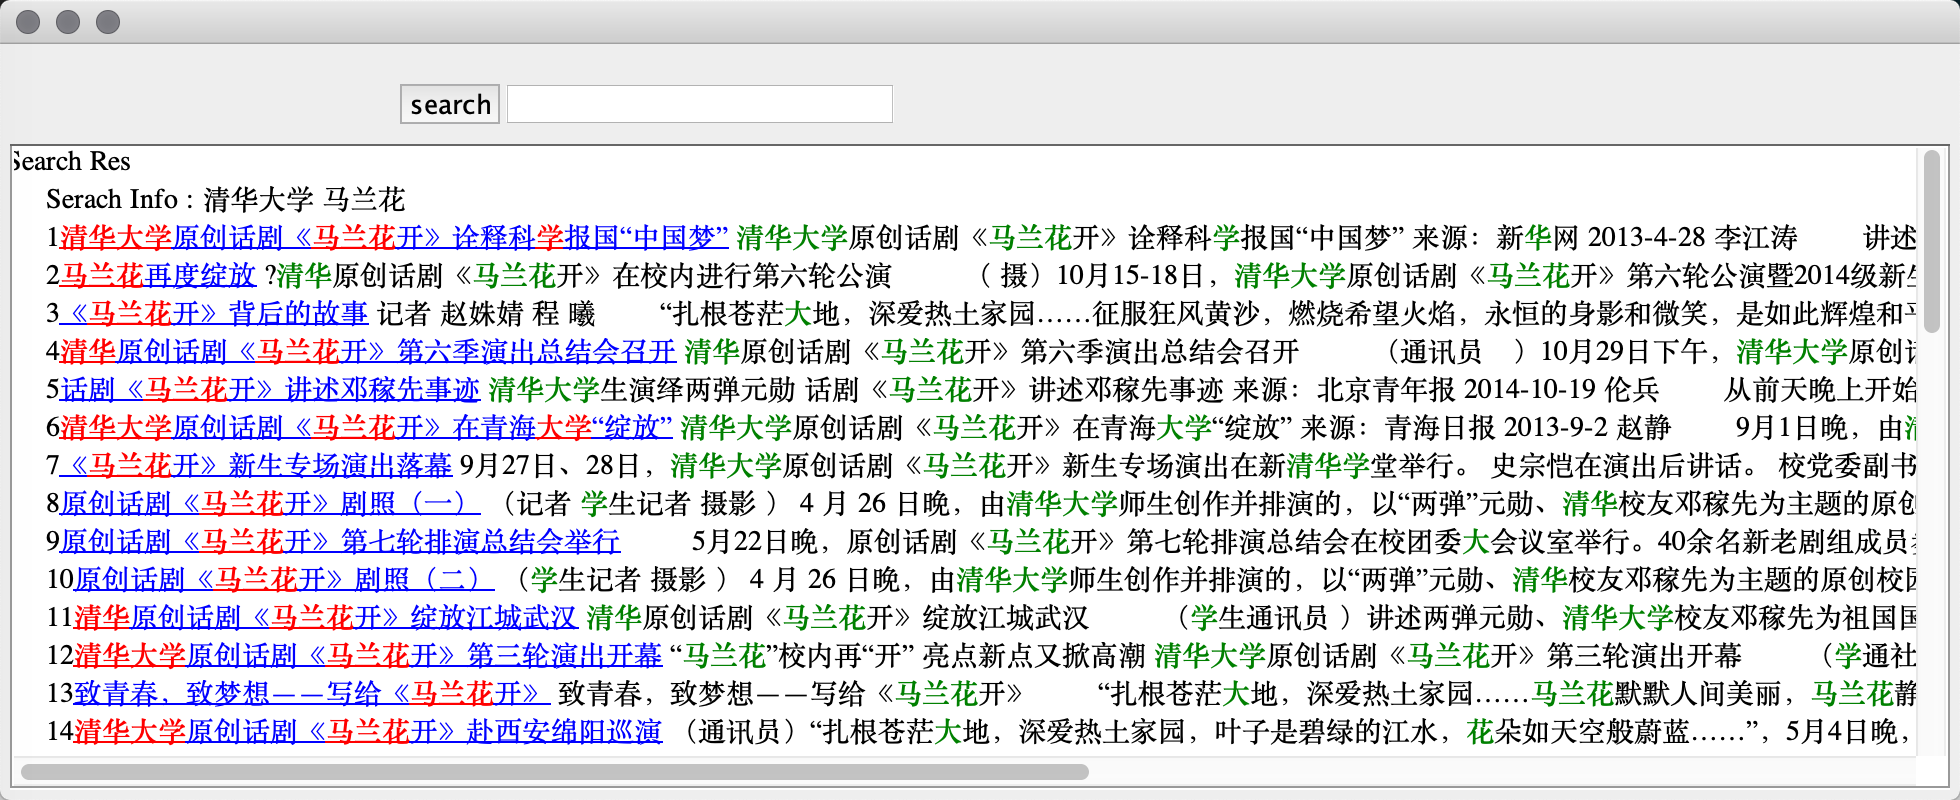
\includegraphics[width=0.9\textwidth]{1.png} 
	\caption{result} 
	\label{img} 
	\end{figure}

	\section{总结}
		本次实验中通过对开源工具的使用节省了大量的处理工作,但在具体的工作中也遇到过很多问 题:Heritrix 的环境搭建与抓取中出现闪退,抓取数据仅几百兆等问题,但通过搜索博客与 同学交流均得到解决并为其他同学提供解答帮助,进一步熟悉了对 Heritrix 的使用和处理。 同时对于分词和解析的工具使用也更熟悉和得心应手。

		\par 
		总体而言,本次试验的收获还是比较大的。
		 
	\bibliographystyle{unsrt}
	\bibliography{reference}
\end{document}

